\documentclass{article}
\usepackage{amsmath, amssymb, graphicx}
\usepackage{afterpage}

\title{Broker Optimisation Algorithm}
\author{Álvaro Rodríguez Gallardo}
\date{\today}

\begin{document}

\maketitle

\section{Introduction}

\section{Algoritmo Genérico y MOEA}

Input al sistema: Lista de funciones de radioastronomía para ejecutar:

\begin{itemize} % Inicio de la lista de funciones
  \item func1
  \item func2
  \item $\ldots$
  \item funcN
\end{itemize} % Fin de la lista de funciones

Se propone un algoritmo grande que utiliza un MOEA (Optimización Multiobjetivo Basada en Evolución) para minimizar el tiempo de ejecución y la energía consumida.

Suponemos un sistema de M nodos.

El flujo del programa sería el siguiente.

\subsection{Algoritmo Genérico}

\begin{verbatim}
BeginProcedure
  matriz_paretos = matrix[N][M]  // {N filas, M columnas}
  
  For{func in lista_funciones} // {Itera sobre la lista de funciones}
    For{nodo in lista_nodos}   // {Itera sobre la lista de nodos}
      lista\_paretos = 'python moea_broker_optimisation.py ${func} ${nodo}'
      matriz_paretos[i][j] = lista_paretos
    EndFor
  EndFor
  
  mejores_nodos = list[N]
  
  For{i in range(len(lista_funciones))}
    mejores_nodos[i] = minimo_pareto_func(matriz_paretos, fila=i)
  EndFor
  
  HACERDECISION(mejores_nodos)
EndProcedure
\end{verbatim}

Este algoritmo no parece ser muy eficiente a primera vista y podría requerir optimización.

\subsection{Algoritmo MOEA por Nodo}

El algoritmo MOEA para cada nodo tendría la siguiente lógica:

\begin{verbatim}
BeginProcedure
  my_function = funcion
  id_nodo = nodo.id
  especificaciones_nodo = nodo.especificaciones
  guardarMaximoCoresCargaNodoDependencias(especificaciones_nodo)
  
  objeto = MOEAForBroker.inicializar(funcion)
  
  lista_resultados_paretos = []  // {Diccionario (algoritmo, resultados algoritmo)}
  
  For{algoritmo_moea in algoritmos_propuestos}
    lista_resultados_un_alg =  objeto.ejecutarAlgoritmoPropuesto(algoritmo_moea)
    lista_resultados_paretos.append('algoritmo_moea': lista_resultados_un_alg)
  EndFor
  
  return lista_resultados_paretos
\EndProcedure
\end{verbatim}

En esta sección, se profundiza en la implementación del modelo que seguirá el MOEA, incluyendo resultados teóricos y estadísticos sobre variables como el número de cores y el tiempo de acceso a datos.

\section{Theorical aspects}

\subsection{Generic algorithm}

\subsection{Execution Time in CPU}

We define $|A|$ as the cardinality of set $A$, representing the number of elements within $A$, which are nodes index where needed data are. Let $tTransf_j$ be the time spent transferring data from node $j \in A$. Suponiendo el caso en que todos los datos necesarios están dentro del nodo en cuestión, debemos tanto acceder a los datos como ejecutar la función. En consecuencia, el tiempo de ejecución será, si \(nCores\) es el número de cores de CPU

\[
tEjec = \frac{1}{nCores}(tAccessData + tProcessingData)
\]

En la expresión anterior, se considera tanto el tiempo de acceso a datos (dependerá del tipo de dato que se quiera obtener) como el tiempo de ejecución de la función de WSClean. También se ha supuesto una ejecución en paralelo, repartiendo el trabajo según \(nCores\), por lo que a mayor número de cores, menor tiempo de ejecución dentro del nodo. Se justifica la elección de la función que modela el comportamiento de los cores más adelante.

Now, let's analyze the situation. Transfer time is assumed to be independent between nodes. We have two cases:

\begin{itemize}
  \item If $nCores$ is fixed, we have a straight line in a $|A|$-dimensional space.
  \item If $nCores$ is variable ($nCores \in \mathbb{N}$), then we have a $|A|+1$-dimensional function, with a vertical asymptote at $nCores=0$. Assuming $nCores$ is not 0 in the CPU, it behaves like a linear function depending on time. We have $|A|+2$ variables.
\end{itemize}

But, in a real situation, we have other type of restrictions, so the number of variables grows.

Ahora se extiende la situación a la falta de datos dentro del nodo y la comunicación de este con otros nodos con los datos necesarios. Se buscará la mínima interacción con nodos ajenos, por lo que el tiempo crecerá cuanto mayor sea la comunicación con nodos. No se pierde generalidad, pues si no hay necesidad de comunicación con otros nodos, los términos añadidos a continuación serán cero.

Considering transmission time and node bandwidth (i.e. MB/s), the execution time in CPU is given by
\[
tEjec = \sum_{j \in A} t_{ij} + \sum_{j \in A} tEjec_j + \sum_{j \in A} t_{ji} + \frac{1}{nCores}(tAccessData + tProcessingData)
\]

where generally \(t_{ij} \neq t_{ji}\) because of node brandwith (it is supposed, if node i brandwith is \(V_i\), then \(t_{ij}=\frac{d_{ij}}{V_i}\) and the same with \(V_j\), where \(d_{ij}=d_{ji}\) is distance between nodes i and j).

Besides, it is added execution time of node j. Same problem can be found in node j: it needs data from other node, or nodes, we say \(k_1,...,k_m\), so function must be recursive to take into account this situation. If it is thought in that as a data structure like a tree, then in a certain moment execution time of other nodes is zero becase that node (leaf) does not need data from other nodes.

Lastly, if node i is executed, and it needs data from node j, then it has been thought in a situation in which node j needs data from node i. It is a particular case of last paragraph, it should not make troubles like eternal loops.

\subsection{Execution Time in General}

As discussed in the document \texttt{Discusion\_uso\_1\_n\_p.pdf}, a function of the form $\frac{1}{nCores^p}$ is proposed for general execution time, where $nCores$ is the number of cores, and $p$ depends on the hardware technology. For example, for CPU, $p=1$. For GPU, $p>1$, such as $p=3$, but the exact value needs thorough study.

In summary, the abstract expression for execution time is
\[
tEjec = \sum_{j \in A} t_{ij} + \sum_{j \in A} tEjec_j + \sum_{j \in A} t_{ji} + \frac{1}{nCores^p}(tAccessData + tProcessingData)
\]

Recalcar que no conocemos \(tAccess\) o \(tProcessingData\) pues antes hay que tener todos los datos de otros nodos dentro del mismo, por lo que esta expresión, al momento de calcularla, debe ir de izquierda a derecha y habiendo calculado antes los sumatorios.

\subsection{Execution Time: Justification depending on used hardware}

\subsubsection{Introduction}

Firstly, we have a problem in which we should use a MultiObjective Evolutionary Algorithm (MOEA). In this first approach, execution time and energy consumption are parameters that should be minimized. Because of that, both objective functions must be defined.

It is going to be justified why $\frac{1}{{x^p}}$ is a good option to model the behavior of CPU or GPU cores (even other hardware components' behavior could be represented this way), but only for execution time

\subsubsection{Mathematical Aspects}

Let \(\forall p \in \mathbb{R^+} \cup \{0\}\) the real numbers succession
\[
\frac{1}{{x^p}}
\]
where $x$ is a positive real number (in the next sections it is related to the quantity of cores).

Later, the number $p$ will tell if the function is associated with a hardware component, and it should be known what its behavior is: if we set a high number of cores in the CPU or GPU, for example, execution time should converge to zero, and the previous function fulfills that.

However, GPU reduces execution time, so number $p$ discriminates which technology is being used. Because of that, let $p$, $q$ be positive real numbers, and some properties should be studied.

\subsubsection{Asymptotic behavior}

It is true that
\[
\lim_{{x \to \infty}} \frac{1}{{x^p}}=\lim_{{x \to \infty}} \frac{1}{{x^q}}=0
\]

\[
\lim_{{x \to 0}} \frac{1}{{x^p}}=\lim_{{x \to 0}} \frac{1}{{x^q}}=\infty
\]

so these properties must be taken into account when other ones have been studied.

\subsubsection{Cut Points}

We suppose $p > q$. Then $\frac{1}{{x^p}}=\frac{1}{x^q}$ $\Leftrightarrow$ ${x^p}={x^q}$ $\Leftrightarrow$ ${x^p}-{x^q}=0$ $\Leftrightarrow$ ${x^q}({x^{p-q}}-1)=0$. As $x>0$, we have
\[
{x^{p-q}}-1=0 \Leftrightarrow {x^{p-q}}=1
\]

If ${p-q} \in \mathbb{N}$, then we have $p-q$ solutions because of the Fundamental Theorem of Algebra. In other case, with some transformations, we get the same case: one of the cut points is 1. The rest of them are complex or negative numbers, so in our future problem, there is only one cut point in $x=1$.

\subsubsection{Monotony}

First of all, let two values, $x=\frac{1}{2}$ and $x=3$
\[
	\frac{1}{\frac{1}{2}^p}={2^p} > \frac{1}{3^p}
\]

Besides, we have
\[
	\frac{d}{dx}\left[ \frac{1}{{x^p}} \right] = \frac{d}{dx}\left[x^{-p} \right] = -p \cdot x^{-p-1} < 0 \textbf{ } \forall x>0 \textbf{ } p\neq 0
\]

so there are no relative extremes, and the function decreases. If \(p = 0\), then our succession is constantly 1.

\subsubsection{Conclusions}

With the previous information, if $p>q$ and if $x=\frac{1}{2}$, $x=3$ then $\frac{1}{\frac{1}{2}^p}={2^p} > \frac{1}{\frac{1}{2}^q}={2^q}$, $\frac{1}{3^p} < \frac{1}{3^q}$, so we can confirm the next

\[
	\frac{1}{{x^p}} > \frac{1}{{x^q}} \textbf{ } if \textbf{ } 0<x<1
\]

\[
	\frac{1}{{x^p}} \leq \frac{1}{{x^q}} \textbf{ } if \textbf{ } x \geq 1
\]

\subsubsection{Graphics}

In this section, it is going to be shown graphically the behavior mentioned above. I use Jupyter Notebook with Python.

For some values, I plot some graphics (in some cases p value, which is not the same p value in Statistic, is higher than q value, I do that because I want to show that in the last section I said p\(>\)q, but it does not matter).

\begin{verbatim}
import matplotlib.pyplot as plt
import numpy as np

# Arrays p_array y q_array
p_array = [1, 2, 3, 4]
q_array = [4, 3, 2, 1]

# Valores de x para las funciones
x_values = np.linspace(0.1, 5, 1000)

# Crear una matriz de subgráficos
fig, axs = plt.subplots(len(p_array), len(q_array), figsize=(15, 10), sharex=True, sharey=True)

for i, p_value in enumerate(p_array):
    for j, q_value in enumerate(q_array):
        # Calcular las funciones 1/x^p y 1/x^q
        y_p = 1 / np.power(x_values, p_value)
        y_q = 1 / np.power(x_values, q_value)
        
        # Graficar las funciones en el subgráfico correspondiente
        axs[i, j].plot(x_values, y_p, color='red', label=f'p_value={p_value}')
        axs[i, j].plot(x_values, y_q, color='blue', label=f'q_value={q_value}')
        
        # Establecer límites de ejes personalizados
        axs[i, j].set_xlim(0, 5)
        axs[i, j].set_ylim(0, 2)
        
        # Agregar etiquetas y leyenda
        axs[i, j].set_title(f'p_value={p_value}, q_value={q_value}')
        axs[i, j].legend()

plt.tight_layout()
plt.show()
\end{verbatim}

Results are

\begin{figure}[h]
  \centering
  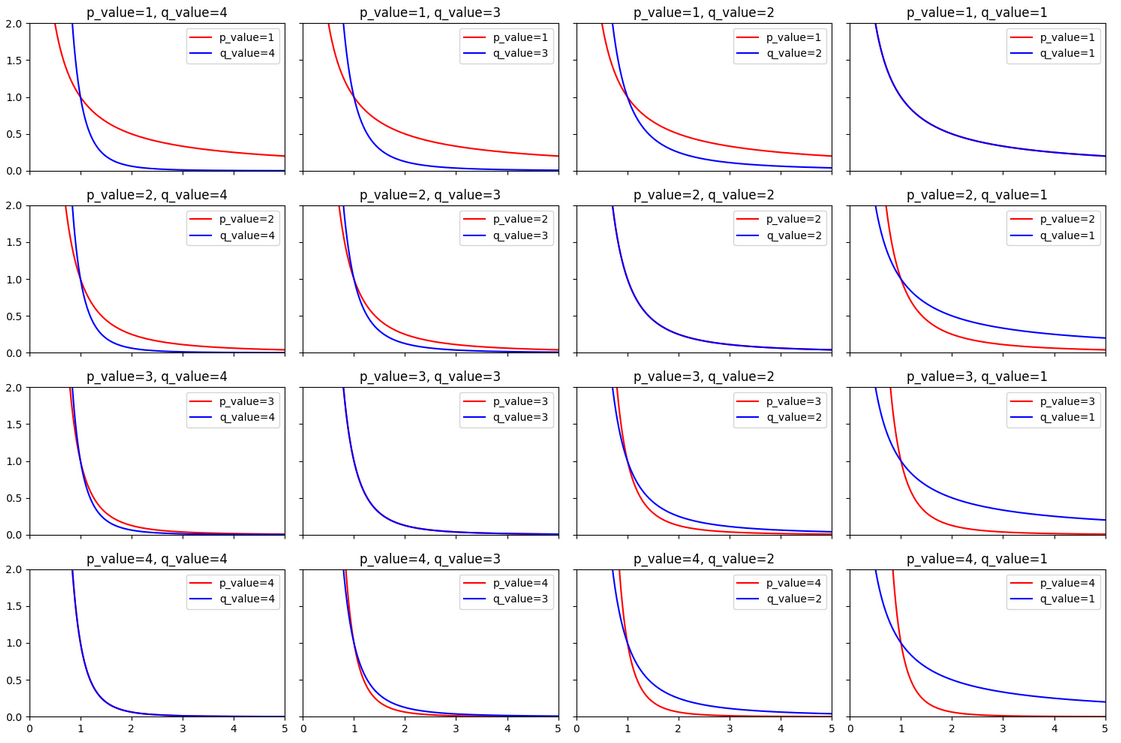
\includegraphics[width=1.3\textwidth]{graficas.png}
  \caption{Graphics in which both functions' behavior is shown}
  \label{fig:etiqueta}
\end{figure}

  \clearpage
  \subsection{Energy Consumption in CPU}
  First of all, in which situations does energy consumption grow? I expose some of them 
  
	\begin{itemize}
       \item More cores \(\implies\) more energy consumption. 
       \item More data to process \(\implies\) more energy consumption (depending on algorithm, quantity of data,...).
       \item "Do I need to convey data to other nodes?" If yes \(\implies\) more energy consumption.
       \item "Do I need data from other nodes?" If yes \(\implies\) more energy consumption (because while node is waiting, it consumes energy).
	\end{itemize}
 It is supposed we want a function that models energy consumption in general, so function must take into account energy consumption of foreign nodes. We use the same set A mentioned above. Then a possible function can be
 
\begin{align*}
    EnConsumption &= EnConsumptionProcessing + \sum_{j \in A} EnConsTransmission_{ij} \\
    &\quad + \sum_{j \in A} EnWaitingNode_j + \sum_{j \in A} EnOtherNode_j
\end{align*}


Here, we have energy consumption in processing data (it includes algorithms used within node, access to data within node,..., it is a variable that must be studied thoroughly). We also have a variable that represents to energy consumed in transmission operations. Then, as it was hypothesized, if node i needs data from other nodes, then it must wait to execution in other nodes, so although consumption i node i does not depend on consumption in other nodes, it depends on how much time node i must wait to operations in other nodes.

Note that function above does not have explicitly number of cores. It may be studied before. For time, it was considered successions of functions \(\{\frac{1}{x^p}\}\). Although \(x^p\), where \(p \in \mathbb{N}\) is an option, and fulfills restrictions on energy consumption in CPU/GPU/ARM, or other hardware components, I do not know if cores function should have a \(x^p\) behaviour

\subsection{Energy Consumption in General}

I have thought in three options:
	\begin{itemize}
		\item If \(f\) is a function that models execution time, then a I have understood, energy consumption has an inverse behaviour. So intuitively, it can be thought we should get a function, let \(g\), with which \(f \circ g =(x_1,...x,_p)\), where \(f\) has p variables. In other words, \(g=f^{.1}\). However, in expression of f (we called it \(tEjec\), none variable can be cleared, that represents energy consumption, at least globally (locally I think we have a dependence between execution time in foreign nodes and energy consumption waiting them). On the other hand, because of implicit functions it is not a feasible option (we do not know how much data from other nodes is needed, so it can be hard to find a goo explicit expression).
		\item We know \(f\) can not be 0, and energy consumption seems to have an inverse behaviour. In this case, and because it seems that energy consumption has the same variables as execution time, but with inverse behaviour, then it is proposed that, if \(g\) represents energy consumption, then \(g = (f)^{-1}=\frac{1}{f}\). It is an option, but not the best (surely other variables or some situations are not taken into account).
		\item Trying to modelise energy consumption as it was made with execution time. In this case, CPU and GPU has an inverse behaviour from execution time, and I think that behaviour is different in this case, so it must be studied thoroughly. I will try to unify hardware behaviour as I did in execution time, studying successions of functions and proposing them as a feasible option.
	\end{itemize}
	\section{Implementation}

Para implementar el algoritmo dado un nodo sobre el que ejecutar la función, se usa Python como lenguaje, apoyado en Platypus para experimentar con diversos algoritmos evolutivos multi-objetivo. Todas las variables necesarias para el correcto funcionamiento, según el marco teórico anterior, son definidas

\begin{verbatim}
	p_CPU = 1
	p_ARM = 2
	p_GPU = 3
	N_execution_plannings = 1 

	max_cpu_cores = 10
	max_gpu_cores = 10
	max_arm_cores = 10
	max_node_in_graph = 40
\end{verbatim}

Se define la clase MOEAforbroker que se apoya en clases padre en Platypus para ejecutar el algoritmo que se le indique, facilitando el solo pensar en la definición del problema, restricciones, función objetivo,... Se expone a continuación

\begin{itemize}
	\item \begin{verbatim} super(MOEAforbroker,self).__init__(P_decision_var,N_functions_tuplas)

	\end{verbatim} Se define el problema. Actualmente, hay tres variables de decisión (cores según hardware) y dos funciones (que queremos minimizar, son el tiempo y la energía)
	\item \begin{verbatim}
	self.types[:] = [Integer(0,max_cpu_cores),Integer(0,max_gpu_cores),
	Integer(0,max_arm_cores)] 
	\end{verbatim} Definición del dominio de las variables de decisión. El máximo de cada dominio será la cantidad máxima de cores disponibles.
	\item \begin{verbatim}
	self.constraints[:] = [not_zero_at_same_time,if_one_positive_rest_zero]
	\end{verbatim}Las restricciones de las soluciones válidas. Como se definen manualmente, Platypus da como válidas aquellas que las funciones devuelve un valor menor o igual a 0. Básicamente, al menos una debe ser positiva, y si una es positiva el resto son cero.
	\item \begin{verbatim}
	self.directions[:] = [Problem.MINIMIZE,Problem.MINIMIZE]
	\end{verbatim} Se indica que queremos minimizar los valores de las funciones objetivo.
\end{itemize}
Además, se penalizan las soluciones con tiempo de ejecución o energía consumida cero, pues en un caso real no puede ocurrir.
\begin{verbatim}
if t_exec<=0.0 or e_consumption<=0.0:   
            t_exec = e_consumption = 1000
\end{verbatim}


\end{document}